% Usage: knitr slide


\chapter{Transformations, Measuring Change, and Regression to the Mean}

\section{Transformations}

\bi
 \item Normality assumption will not always hold
 \bi
  \item Skewed distribution
  \item Different standard deviation in different groups
 \ei
 \item Transforming data can be a simple method to overcome these problems
 \item Non-parametric methods (Wilcoxon signed rank, Wilcoxon rank
   sum) another good option
\ei


\section{Logarithmic Transformation}

\bi
\item Replace individual value by its logarithm
  \bi
   \item $u = log(x)$
  \ei
\item In statistics, always use the \textit{natural} logarithm (base
  $e$; $ln(x)$)
\item Algebra reminders
  \bi
  \item $log(ab) = log(a) + log(b)$
  \item $log\left(\frac{a}{b}\right) = log(a) - log(b)$
  \item Inverse of the log function is $exp(u) = x$, where $exp(u) =
    e^{u}$ and $e$ is a constant ($e = 2.718282 ...$)
  \ei
\ei

\subsection{Example Dataset}

\bi
  \item From Essential Medical Statistics, 13.2 (pre data only)
  \item Response: Urinary $\beta$-thromboglobulin ($\beta$-TG)
    excretion in 24 subjects
  \item 24 total subjects: 12 diabetic, 12 normal
\ei

\begin{Schunk}
\begin{Sinput}
d <- rbind(
  data.frame(status='normal',
             btg=c(4.1, 6.3, 7.8, 8.5, 8.9, 10.4, 11.5, 12.0, 13.8,
                   17.6, 24.3, 37.2)),
  data.frame(status='diabetic',
             btg=c(11.5, 12.1, 16.1, 17.8, 24.0, 28.8, 33.9, 40.7,
                   51.3, 56.2, 61.7, 69.2)))
require(ggplot2)
require(data.table)
\end{Sinput}
\begin{Sinput}
d <- data.table(d)
meds <- d[, j=list(btg = median(btg)), by = status]
p1 <- 
  ggplot(d, aes(x=status, y=btg)) +    # Fig. (*\ref{fig:change-diabetes}*)
  geom_dotplot(binaxis='y', stackdir='center', position='dodge') +
  geom_errorbar(aes(ymin=..y.., ymax=..y..), width=.25, size=1.3, data=meds) +
   xlab('') + ylab(expression(paste(beta-TG, ' (ng/day/100 ml creatinine)'))) + 
  coord_flip()
p2 <- ggplot(d, aes(x=status, y=btg)) +
  scale_y_log10(breaks=c(4,5,10,15,20,30,40,60,80)) +
  geom_dotplot(binaxis='y', stackdir='center', position='dodge') +
  xlab('') + ylab(expression(paste(beta-TG, ' (ng/day/100 ml creatinine)'))) +
  coord_flip()
arrGrob(p1, p2, ncol=2)
\end{Sinput}
\begin{figure}[htbp]

\centerline{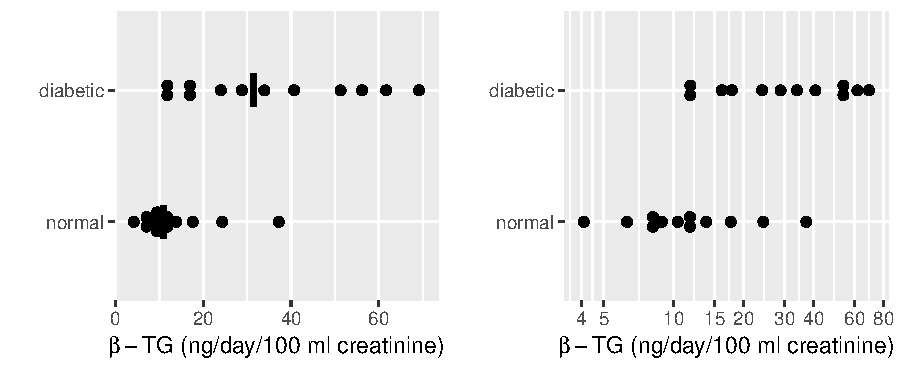
\includegraphics{change-diabetes-1} }

\caption[$\beta$-TG levels by diabetic status]{$\beta$-TG levels by diabetic status with a median line.  The left plot is on the original (non-transformed) scale and includes median lines.  The right plot displays the data on a log scale.}\label{fig:change-diabetes}
\end{figure}
\end{Schunk}
\bi
 \item Original scale
  \bi
   \item Normal: $\overline{x}_1 = 13.53$, $s_1 = 9.194$, $n_1 = 12$
   \item Diabetic: $\overline{x}_2 = 35.28$, $s_2 = 20.27$, $n_2 = 12$
  \ei
 \item Logarithm scale
  \bi
   \item Normal: $\overline{x}_1^* = 2.433$, $s_1^* = 0.595$, $n_1 = 12$
   \item Diabetic: $\overline{x}_2^* = 3.391$, $s_2^* = 0.637$, $n_2 = 12$
  \ei
  \item $t$-test on log-transformed data
  \bi
    \item $s_{pool} = \sqrt{\frac{11 \times .595^2 + 11 \times .637^2}{22}} = 0.616$
    \item $t = \frac{2.433-3.391}{0.616\sqrt{1/12 + 1/12)}} = -3.81$, $\textrm{df} = 22$,  $p = 0.001$
  \ei

  \item Confidence Intervals (0.95 CI)
    \bi
     \item Note that $t_{.975,22} = 2.074$
     \item For Normal subjects, a CI for the mean log $\beta$-TG is
      \beqa
        0.95 \textrm{ CI } & = & 2.433 - 2.074 \times \frac{0.595}{\sqrt{12}} \textrm{ to } 2.433 + 2.074 \frac{0.595}{\sqrt{12}} \\
                         & = & 2.08 \textrm{ to } 2.79
      \eeqa
     \item Can transform back to original scale by using the antilog
       function $e(u)$ to estimate \textbf{medians}
	\beqa
            \textrm{Geometric mean} & = & e^{2.433} = 11.39 \\
            0.95 \textrm{ CI } & = & e^{2.08} \textrm{ to } e^{2.79} \\
                               & = & 7.98 \textrm{ to } 16.27 \\
       \eeqa
     \ei
\begin{Schunk}
\begin{Sinput}
t.test(btg ~ status, data=d)
\end{Sinput}
\begin{Soutput}

	Welch Two Sample t-test

data:  btg by status
t = -3.3838, df = 15.343, p-value = 0.003982
alternative hypothesis: true difference in means is not equal to 0
95 percent confidence interval:
 -35.41024  -8.07309
sample estimates:
  mean in group normal mean in group diabetic 
              13.53333               35.27500 
\end{Soutput}
\begin{Sinput}
t.test(log(btg) ~ status, data=d)
\end{Sinput}
\begin{Soutput}

	Welch Two Sample t-test

data:  log(btg) by status
t = -3.8041, df = 21.9, p-value = 0.0009776
alternative hypothesis: true difference in means is not equal to 0
95 percent confidence interval:
 -1.4792986 -0.4352589
sample estimates:
  mean in group normal mean in group diabetic 
              2.433349               3.390628 
\end{Soutput}
\end{Schunk}
  \item Could also use a non-parametric test (Wilcoxon rank sum)
\begin{Schunk}
\begin{Sinput}
wilcox.test(btg ~ status, data=d)
\end{Sinput}
\begin{Soutput}

	Wilcoxon rank sum test with continuity correction

data:  btg by status
W = 18.5, p-value = 0.002209
alternative hypothesis: true location shift is not equal to 0
\end{Soutput}
\begin{Sinput}
wilcox.test(log(btg) ~ status, data=d)
\end{Sinput}
\begin{Soutput}

	Wilcoxon rank sum test with continuity correction

data:  log(btg) by status
W = 18.5, p-value = 0.002209
alternative hypothesis: true location shift is not equal to 0
\end{Soutput}
\end{Schunk}
  \item Note that non-parametric test is the same for the log-transformed outcomes
\ei


\subsection{Limitations of log transformations}
\bi
  \item Can only be used on positive numbers
   \bi
    \item Sometimes use $u = log(x+1)$
   \ei
  \item Is very arbitrary to the choice of the origin
  \item Not always useful or the best transformation
  \item Sometimes use a dimensionality argument, e.g., take cube root
    of volume measurements or per unit of volume counts like blood counts
  \item Cube and square roots are fine with zeros
\ei

\section{Analysis of Paired Observations}
\bi
\item   Frequently one makes multiple observations on same
experimental unit
\item   Can't analyze as if independent
\item   When two observations made on each unit (e.g., pre--post),
        it is common to summarize each pair using a measure of effect
        $\rightarrow$ analyze effects as if (unpaired) raw data
\item   Most common: simple difference, ratio, percent change
\item   Can't take effect measure for granted
\item   Subjects having large initial values may have largest
        differences
\item   Subjects having very small initial values may have
        largest post/pre ratios
\ei

\section{What's Wrong with Change in General?}\label{sec:changegen}
\subsection{Change from Baseline in Randomized Studies}
Many authors and pharmaceutical clinical trialists make the mistake of analyzing change from baseline instead of making the raw follow-up measurements the primary outcomes, covariate-adjusted for baseline.  The purpose of a parallel-group randomized clinical trial is to compare the parallel groups, not to compare a patient with herself at baseline. The central question is for two patients with the same pre measurement value of x, one given treatment A and the other treatment B, will the patients tend to have different post-treatment values? This is exactly what analysis of covariance assesses.  Within-patient change is affected strongly by regression to the mean and measurement error.  When the baseline value is one of the patient inclusion/exclusion criteria, the only meaningful change score requires one to have a second baseline measurement post patient qualification to cancel out much of the regression to the mean effect.  It is the second baseline that would be subtracted from the follow-up measurement.

The savvy researcher knows that analysis of covariance is required to ``rescue'' a change score analysis. This effectively cancels out the change score and gives the right answer even if the slope of post on pre is not 1.0. But this works only in the linear model case, and it can be confusing to have the pre variable on both the left and right hand sides of the statistical model. And if $Y$ is ordinal but not interval-scaled, the difference in two ordinal variables is no longer even ordinal.  Think of how meaningless difference from baseline in ordinal pain categories are. A major problem in the use of change score summaries, even when a correct analysis of covariance has been done, is that many papers and drug product labels still quote change scores out of context.  Patient-reported outcome scales with floor or ceiling effects are particularly problematic.  Analysis of change loses the opportunity to do a robust, powerful analysis using a covariate-adjusted ordinal response model such as the proportional odds or proportional hazards model.  Such ordinal response models do not require one to be correct in how to transform $Y$.


Not only is it very problematic to analyze change scores in parallel group designs; it is problematic to even compute them.  To compute change scores requires many assumptions to hold, e.g.:
\be
\item the variable is not used as an inclusion/exclusion criterion for the study, otherwise regression to the mean will be strong
\item if the variable is used to select patients for the study, a second post-enrollment baseline is measured and this baseline is the one used for all subsequent analysis
\item the post value must be linearly related to the pre value
\item the variable must be perfectly transformed so that subtraction "works" and the result is not baseline-dependent
\item the variable must not have floor and ceiling effects
\item the variable must have a smooth distribution
\item the slope of the pre value vs.\ the follow-up measurement must be close to 1.0 when both variables are properly transformed (using the same transformation on both)
\ee

Details about problems with analyzing change may be found \href{http://biostat.mc.vanderbilt.edu/MeasureChange}{here}, and references may be found \href{http://www.citeulike.org/user/harrelfe/tag/change}{here}.

Regarding 3. above, if pre is not linearly related to post, there is no transformation that can make a change score work.  Two unpublished examples illustrate this problem.  In a large degression study using longitudinal measurements of the Hamilton-D depression scale, there was a strong nonlinear relationship between baseline Hamilton D and the final measurement.  The form of the relationship was a flattening of the effect for larger Ham D, indicating there are patients with severe depression at baseline who can achieve much larger reductions in depression than an average change score would represent (and likewise, patients with mild to moderate depression at baseline would have a reduction in depression symptoms that is far less than the average change indicates).  Doing an ordinal ANCOVA adjusting for a smooth nonlinear effect of baseline using a spline function would have been a much better analysis than the change from baseline analysis done by study leaders.  In the second example, a similar result was found for a quality of life measure, KCCQ.  Again, a flattening relationship for large KCCQ indicated that subtracting from baseline provided a nearly meaningless average change score.

Regarding 7. above, often the baseline is not as relevant as thought and the slope will be less than 1.  When the treatment can cure every patient, the slope will be zero.  When the baseline variable is irrelevant, ANCOVA will estimate a slope of approximately zero and will effectively ignore the baseline.  Change will baseline will make the change score more noisy than just analyzing the final raw measurement.  In general, when the relationship between pre and post is linear, the correlation between the two must exceed 0.5 for the change score to have lower variance than the raw measurement.

Bland and Altman~\cite{bla11com} have an excellent \href{https://www.ncbi.nlm.nih.gov/pmc/articles/PMC3286439}{article} about how misleading change from baseline is for clinical trials.  \href{http://www.fharrell.com/2017/04/statistical-errors-in-medical-literature.html#change}{This} blog article has several examples of problematic change score analyses in the clinical trials literature.

The following \R\ code exemplifies how to do a powerful, robust analysis without computing change from baseline.  This analysis addresses the fundamental treatment question posed at the top of this section.  This example uses a semiparametric ANCOVA that utilizes only the ranks of $Y$ and that provides the same test statistic no matter how $Y$ is transformed.  It uses the proportional odds model, with no binning of $Y$, using the \co{rms} package \co{orm} function\footnote{\co{orm} can easily handle thousands of intercepts (thousands of distinct $Y$ values).}.  This is a generalization of the Wilcoxon test---it would be almost identical to the Wilcoxon test had the baseline effect been exactly flat.  Note that the proportional odds assumption is more likely to be satisfied than the normal residual, equal variance assumption of the ordinary linear model.

\begin{Schunk}
\begin{Sinput}
require(rms)
# Fit a smooth flexible relationship with baseline value y0
# (restricted cubic spline function with 4 default knots)
f <- orm(y ~ rcs(y0, 4) + treatment)
f
anova(f)
# Estimate mean y as a function of y0 and treatment
M <- Mean(f)   # creates R function to compute the mean
plot(Predict(f, treatment, fun=M))  # y0 set to median since not varied
# To allow treatment to interact with baseline value in a general way:
f <- orm(y ~ rcs(y0, 4) * treatment)
plot(Predict(f, y0, treatment))  # plot y0 on x-axis, 2 curves for 2 treatments
# The above plotted the linear predictor (log odds); can also plot mean
\end{Sinput}
\end{Schunk}

\subsection{Special Problems Caused By Non-Monotonic Relationship With Ultimate Outcome}
Besides the strong assumptions made about how variables are
transformed before a difference is calculated, there are many types of
variables for which change can never be interpreted without reference
to the starting point, because the relationship between the variable
in question and an ultimate outcome is not even monotonic.  A good
example is the improper definitions of acute kidney injury (AKI) that have
been accepted without question.  Many of the definitions are based on
change in serum creatinine (SCr).  Problems with the definitions include
\be
\item The non-monotonic relationship between SCr and mortality
  demonstrates that it is not healthy to have very low SCr.  This implies
  that increases in SCr for very low starting SCr may not be harmful as assumed in definitions of AKI.
\item Given an earlier SCr measurement and a current SCr, the earlier
  measurement is not very important in predicting mortality once one
  adjusts for the last measurement.  Hence a change in SCr is not very
  predictive and the current SCr is all-important.
\ee
As an example consider the estimated relationship between baseline SCr
and mortality in critically ill ICU patients.
\begin{Schunk}
\begin{Sinput}
require(rms)
\end{Sinput}
\begin{Sinput}
load('~/Analyses/SUPPORT/combined.sav')
combined <- subset(combined,
  select=c(id, death, d.time, hospdead, dzgroup, age, raceh, sex))
load('~/Analyses/SUPPORT/combphys.sav')
combphys <- subset(combphys, !is.na(crea1+crea3),
                   select=c(id,crea1,crea3,crea7,crea14,crea25,alb3,
                     meanbp3,pafi3,wblc3))
w <- merge(combined, combphys, by='id')
u <- 'mg/dl'
w <- upData(w, labels=c(crea1='Serum Creatinine, Day 1',
                 crea3='Serum Creatinine Day 3',
                 crea14='Serum Creatinine Day 14'),
            units=c(crea1=u, crea3=u, crea7=u, crea14=u, crea25=u))
\end{Sinput}
\begin{Soutput}
Input object size:	 1656136 bytes;	 17 variables	 10279 observations
New object size:	1657176 bytes;	17 variables	10279 observations
\end{Soutput}
\begin{Sinput}
w <- subset(w, crea1 < 2)
dd <- datadist(w); options(datadist='dd')

h <- lrm(hospdead ~ rcs(crea1, 5) + rcs(crea3, 5), data=w)
anova(h)   # (*\label{pg:change-anova}*)
\end{Sinput}
\begin{Soutput}
                Wald Statistics          Response: hospdead 

 Factor          Chi-Square d.f. P     
 crea1            19.52     4    0.0006
  Nonlinear       15.60     3    0.0014
 crea3           108.11     4    <.0001
  Nonlinear       49.98     3    <.0001
 TOTAL NONLINEAR 132.06     6    <.0001
 TOTAL           217.11     8    <.0001
\end{Soutput}
\begin{Sinput}
h <- lrm(hospdead ~ sex * rcs(crea3, 5), data=w)
p <- Predict(h, crea3, sex, fun=plogis)
ggplot(p, ylab='Risk of Hospital Death')    # Fig. (*\ref{fig:change-suppcr}*)
\end{Sinput}
\begin{figure}[htbp]

\centerline{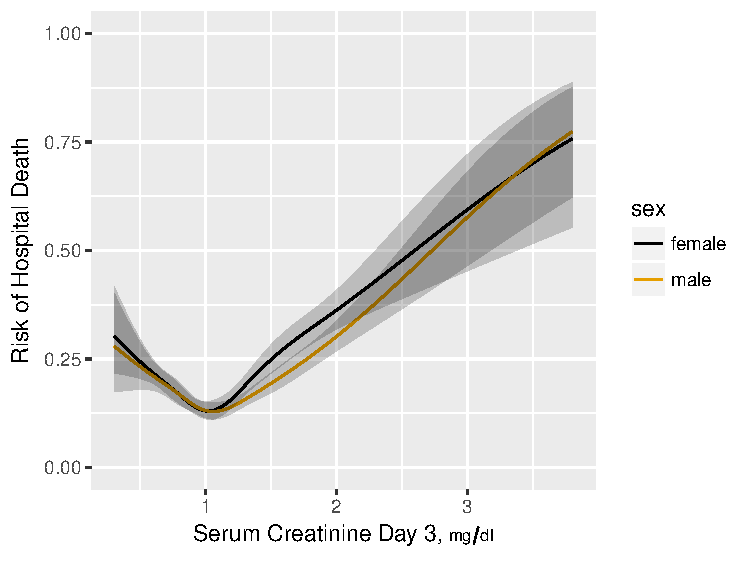
\includegraphics{change-suppcr-1} }

\caption[Hospital death as a function of creatinine]{Estimated risk of hospital death as a function of day 3 serum creatinine and sex for 7772 critically ill ICU patients having day 1 serum creatinine $< 2$ and surviving to the start of day 3 in the ICU}\label{fig:change-suppcr}
\end{figure}
\end{Schunk}
We see that the relationship is very non-monotonic so that it is
impossible for change in SCr to be relevant by itself unless the study
excludes all patients with SCr $< 1.05$.  To put this in perspective,
in the NHANES study of asymptomatic subjects, a very significant
proportion of subjects have SCr $< 1$.


\section{What's Wrong with Percent Change?}
\bi
\item   Definition

\beq
 \% \textrm{ change } = \frac{\textrm{first value} - \textrm{second value}}{\textrm{second value}} \times 100
\eeq
\item The first value is often called the new value and the second value is called the old value, but this does not fit all situations
\item   Example
  \bi
  \item      Treatment A: 0.05 proportion having stroke
  \item      Treatment B: 0.09 proportion having stroke
  \ei
\item The point of reference (which term is used in the denominator?) will impact the answer
  \bi
   \item      Treatment A reduced proportion of stroke by 44\%
   \item      Treatment B increased proportion by 80\%
  \ei
\item   Two increases of 50\% result in a total increase of 125\%, not
        100\%
  \bi
   \item Math details: If $x$ is your original amount, two increases of 50\% is $x*1.5*1.5$. Then, \% change = $(1.5*1.5* x - x) / x = x*(1.5*1.5 - 1) / x = 1.25$, or a 125\% increase
  \ei
\item   Percent change (or ratio) not a symmetric measure
  \bi
  \item A 50\% increase followed by a 50\% decrease results in an overall decrease (not no change)
   \bi
    \item Example: 2 to 3 to 1.5
   \ei
  \item A 50\% decrease followed by a 50\% increase results in an overall decrease (not no change)
   \bi
   \item Example: 2 to 1 to 1.5
   \ei
  \ei
\item Unless percents represent proportions times 100, it is not appropriate to compute descriptive statistics (especially the mean) on percents.
  \bi
    \item For example, the correct summary of a 100\% increase and a 50\% decrease, if they both started at the same point, would be 0\% (not 25\%).
  \ei
\item   Simple difference or log ratio are symmetric
\ei

\section{Objective Method for Choosing Effect Measure}
\bi
\item   Goal: Measure of effect should be as independent of
        baseline value as possible\footnote{Because of regression to
        the mean, it may be impossible to make the measure of change
        truly independent of the initial value.  A high initial value
        may be that way because of measurement error.  The high value will
        cause the change to be less than it would have been had the
        initial value been measured without error.  Plotting
        differences against averages rather than against initial
        values will help reduce the effect of regression to the mean.}
\item   Plot difference in pre and post values vs. the pre values.  If this shows no trend, the simple
        differences are adequate summaries of the effects, i.e., they
        are independent of initial measurements.
\item   If a systematic pattern is observed, consider repeating the
        previous step after taking logs of both the pre and post
        values.  If this removes any systematic relationship between
        the baseline and the difference in logs, summarize the data
        using logs, i.e., take the effect measure as the log ratio.
\item   Other transformations may also need to be examined
\ei


\section{Example Analysis: Paired Observations}

\subsection{Dataset description}
\bi
  \item Dataset is an extension of the diabetes dataset used earlier in this chapter
  \item Response: Urinary $\beta$-thromboglobulin ($\beta$-TG) excretion in 24 subjects
  \item 24 total subjects: 12 diabetic, 12 normal
  \item Add a ``post'' measurement (previous data considered the ``pre'' measurement)
\ei

\subsection{Example Analysis}
\begin{Schunk}
\begin{Sinput}
# Now add simulated some post data to the analysis of beta TG data
# Assume that the intervention effect (pre -> post effect) is
# multiplicative (x 1/4) and that there is a multiplicative error
# in the post measurements
set.seed(13)
d$pre  <- d$btg
d$post <- exp(log(d$pre) + log(.25) + rnorm(24, 0, .5))
# Make plots on the original and log scales
p1 <- ggplot(d, aes(x=pre, y=post - pre, color=status)) +
  geom_point() + geom_smooth() + theme(legend.position='bottom')
# Use problematic asymmetric % change
p2 <- ggplot(d, aes(x=pre, y=100*(post - pre)/pre,
                    color=status)) + geom_point() + geom_smooth() +
      xlab('pre') + theme(legend.position='none') +
      ylim(-125, 0)
p3 <- ggplot(d, aes(x=pre, y=log(post / pre),
                    color=status)) + geom_point() + geom_smooth() +
      xlab('pre') + theme(legend.position='none') + ylim(-2.5, 0)
arrGrob(p1, p2, p3, ncol=2)   # Fig. (*\ref{fig:change-analysis}*)
\end{Sinput}
\begin{Sinput}
with(d, {
     print(t.test(post - pre))
     print(t.test(100*(post - pre) / pre))       # improper
     print(t.test(log(post / pre)))
     print(wilcox.test(post - pre))
     print(wilcox.test(100*(post - pre) / pre))  # improper
     print(wilcox.test(log(post / pre)))
     } )
\end{Sinput}
\begin{Soutput}

	One Sample t-test

data:  post - pre
t = -5.9366, df = 23, p-value = 4.723e-06
alternative hypothesis: true mean is not equal to 0
95 percent confidence interval:
 -22.68768 -10.96215
sample estimates:
mean of x 
-16.82492 


	One Sample t-test

data:  100 * (post - pre)/pre
t = -23.864, df = 23, p-value < 2.2e-16
alternative hypothesis: true mean is not equal to 0
95 percent confidence interval:
 -75.19217 -63.19607
sample estimates:
mean of x 
-69.19412 


	One Sample t-test

data:  log(post/pre)
t = -13.147, df = 23, p-value = 3.5e-12
alternative hypothesis: true mean is not equal to 0
95 percent confidence interval:
 -1.483541 -1.080148
sample estimates:
mean of x 
-1.281845 


	Wilcoxon signed rank test

data:  post - pre
V = 0, p-value = 1.192e-07
alternative hypothesis: true location is not equal to 0


	Wilcoxon signed rank test

data:  100 * (post - pre)/pre
V = 0, p-value = 1.192e-07
alternative hypothesis: true location is not equal to 0


	Wilcoxon signed rank test

data:  log(post/pre)
V = 0, p-value = 1.192e-07
alternative hypothesis: true location is not equal to 0
\end{Soutput}
\begin{figure}[htbp]

\centerline{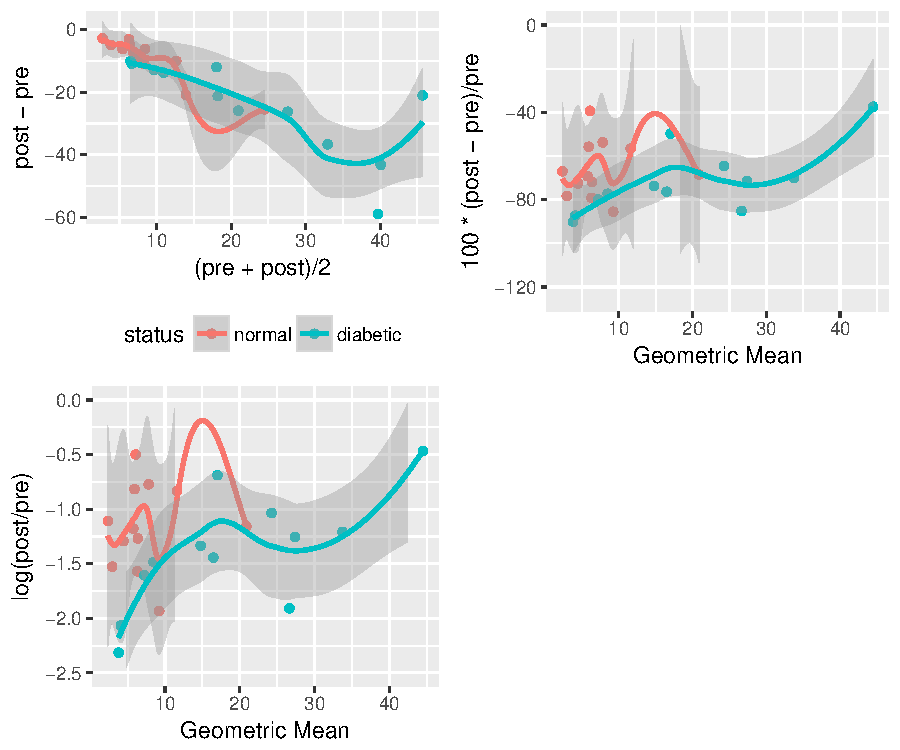
\includegraphics{change-analysis-1} }

\caption[Difference vs]{Difference vs.\ baseline plots for three transformations}\label{fig:change-analysis}
\end{figure}
\end{Schunk}
\textbf{Note}: In general, the three Wilcoxon signed-rank statistics
will not agree on each other.  They depend on the symmetry of the
difference measure.
\nocite{kai89,tor85how,mar85mod,kro93spu,col00sym}

\section{Regression to the Mean}\label{sec:change-rttm}\movie{https://youtu.be/yWoKLDy8IQA}
\bi
\item One of the most important of all phenomena regarding data and estimation
\item Occurs when subjects are selected because of their values
\item Examples:
 \be
 \item Intersections with frequent traffic accidents will have fewer accidents in the next observation
  period if no changes are made to the intersection
 \item The surgeon with the highest operative mortality will have a
   significant decrease in mortality in the following year
 \item Subjects screened for high cholesterol to qualify for a clinical trial will have lower
  cholesterol once they are enrolled
 \ee
\item Observations from a randomly chosen subject are unbiased for that subject
\item But subjects \emph{selected} because they are running high or low are selected partially because
  their measurements are atypical for themselves (i.e., selected \emph{because} of measurement error)
\item Future measurements will ``regress to the mean'' because measurement errors are random
\item For a classic misattribution of regression to the mean to a
  treatment effect see
  \href{https://www.advisory.com/Daily-Briefing/2013/09/30/How-a-hospital-used-social-workers-to-cut-readmissions}{this}\footnote{In
    their original study, the social workers enrolled patients having 10 or 
  more hospital admissions in the previous year and showed that after
  their counseling, the number of admissions in the next year was less than
  10.  The same effect might have been observed had the social workers
  given the patients horoscopes or weather forecasts.  This was
  reported in an abstract for the AHA meeting that has since been
  taken down from \url{circ.ahajournals.org}.}.
\ei

Classic paper on shrinkage: Efron \& Morris~\cite{efr77sti}
\bi
\item Shrinkage is a way of discounting observed variation that accounts for regression to the mean
\item In their example you can see that the variation in batting averages for the first 45 at bats is
  unrealistically large
\item Shrunken estimates (middle) have too little variation but this discounting made the estimates closer
  to the truth (final batting averages at the end of the season)
\item You can see the regression to the mean for the \emph{apparently}
  very hot and very cold hitters
\ei
\begin{Schunk}
\begin{Sinput}
nam <- c('Roberto Clemente','Frank Robinson','Frank Howard','Jay Johnstone',
  	 'Ken Berry','Jim Spencer','Don Kessinger','Luis Alvarado',
		 'Ron Santo','Ron Swoboda','Del Unser','Billy Williams',
		 'George Scott','Rico Petrocelli','Ellie Rodriguez',
		 'Bert Campaneris','Thurman Munson','Max Alvis')
initial <- c(18,17,16,15,14,14,13,12,11,11,10,10,10,10,10,9,8,7)/45
season  <- c(345,297,275,220,272,270,265,210,270,230,265,258,306,265,225,
             283,320,200)/1000
initial.shrunk <- c(294,288,280,276,275,275,270,265,262,263,258,256,
                    257,256,257,252,245,240)/1000
plot(0,0,xlim=c(0,1),ylim=c(.15,.40),type='n',axes=F,xlab='',ylab='')
n  <- 18
x1 <- .5
x2 <- .75
x3 <- 1
points(rep(x1,n), initial)
points(rep(x2,n), initial.shrunk)
points(rep(x3,n), season)

for(i in 1:n) lines(c(x1,x2,x3),c(initial[i],initial.shrunk[i],season[i]),
                    col=i, lwd=2.5)
axis(2)
par(xpd=NA)
text(c(x1,x2+.01, x2+.25),rep(.12,3),c('First 45 ABs','Shrunken\nEstimates',
     'Rest of\nSeason'))
for(a in unique(initial)) {
  s <- initial==a
  w <- if(sum(s) < 4) paste(nam[s],collapse=', ') else {
	j <- (1:n)[s]
	paste(nam[j[1]],', ',nam[j[2]],', ',nam[j[3]],'\n',
		  nam[j[4]],', ',nam[j[5]],sep='')
  }
  text(x1-.02, a, w, adj=1, cex=.9)
}
\end{Sinput}
\begin{figure}[htbp]

\centerline{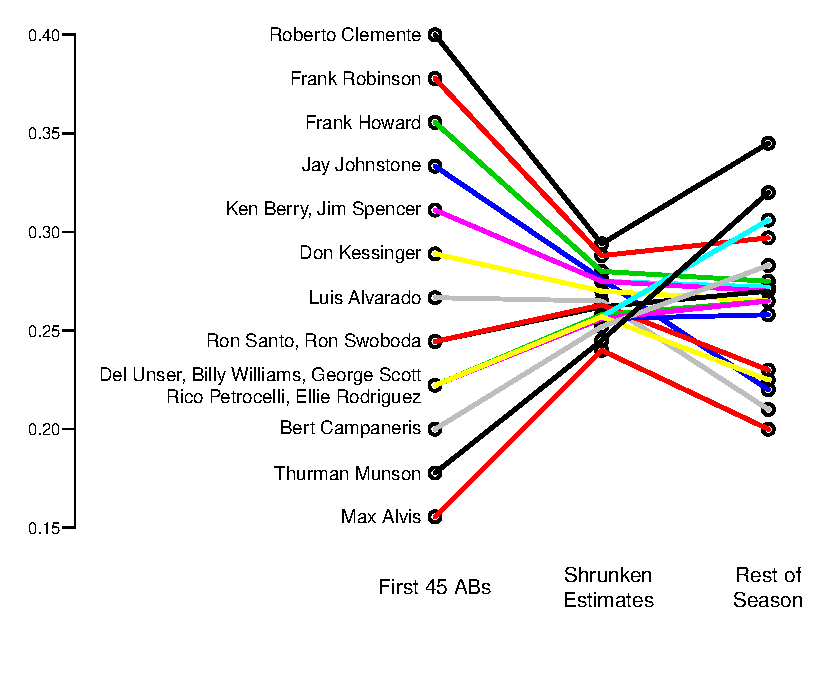
\includegraphics{change-baseball-1} }

\caption[Baseball batting averages and regression to the mean]{Initial batting averages as estimates of final batting averages for players, along with shrunken estimates that account for regression to the mean}\label{fig:change-baseball}
\end{figure}
\end{Schunk}
